\section{分次环的\texorpdfstring{$\proj$}{Proj}}\label{s:3.2}

\subsection{\texorpdfstring{$\proj S$}{Proj S}的构造}\label{s:3.2.1}

到目前为止,非仿射概形最重要的例子是在一个仿射概形$\spec A$上的\textit{射影}概形,其中$A$是任意一个交换环。(为简单起见,我们常常说一个概形在$A$上射影,而不说在$\spec A$上射影。)这样的一个概形来自于一个分次$A$-代数,而构造过程非常类似于从它的齐次坐标环构造一个射影簇。我们可以从一个分次$\oo_B$-代数层开始,定义在任意的基概形$\spec B$上射影的概形,这个拓展有重要的应用。但对这个理论中的大部分情况而言,我们都可以将情况约化到$B$是一个仿射概形,故而在这里,我们对一般性的追求也仅止于此。

为了描述这个构造,我们从一个正分次$A$-代数开始,其中$A$作为这个代数的$0$次部分,即一个$A$代数$S$具有分次
\[
	S=\bigoplus_{\nu=0}^\infty S_\nu\quad \text{作为$A$-模}
\]
使得
\[
	S_\nu S_\mu \subset S_{\nu+\mu}\quad \text{以及} \quad S_0=A.
\]
$S$中的一个元素如果处于$S_\nu$中,则它被称为$\nu$\textit{次齐次}的。我们将从$S$定义一个$A$-概形$X=\proj S$. 在$A$上射影的概形就被定义为具有形式$\proj S$的概形,其中$S$是一个有限生成$A$-代数。代数$S$被称为$X$的\textit{齐次坐标环},尽管(类似于射影簇的齐次坐标环)实际上他并不由$X$所决定。

当$S$是$A$上的多项式环
\[
	S=A[\text{$x_0$, $\dots$, $x_r$}],
\]
具有如下分次:$A$中的元素是零次的,而每一个变量的分次都是$1$,则给出的概形$\proj S$被称为\textit{$A$上的射影$r$-空间},记作$\mathbb{P}_A^r$.(后面的习题将说明这个概形与第 \ref{chap:1} 章中定义的概形$\mathbb{P}_A^r$是相同的。)在$A=K$是一个域的例子中,概形$\mathbb P_K^r$与$K$上的名为射影空间的簇之间的关系就类似于概形$\mathbb A_K^r$与名为仿射$r$-空间的簇之间的关系。

为方便起见,我们将假设代数$S$在$A$上被它的$1$-次元素所生成,类似于多项式环那样,一般的情况我们留做习题。(换个方向,如果$S$并没有假设在$A$上有限生成,下面我们说的绝大部分内容依然成立,但这种推广用得相对较少)。

$\proj S$可以如下定义:对$S$中的正次齐次元生成的理想,我们记
\[
	S_+=\bigoplus_{\mu=1}^\infty S_\mu.
\]
我们称一个理想是\textit{齐次}的如果它由齐次元所生成。底空间$|\proj S|$是环$S$中所有不包含$S_+$的齐次素理想的集合(它们有时候被叫做\textit{相关}素理想,而$S_+$因此被叫做\textit{无关理想})。$|\proj S|$上的拓扑通过闭集定义,闭集取做形如
\[
	V(I):=\{\pp\,|\,\text{$\pp$是$S$的包含$I$的相关素理想}\}
\]
的集合,其中$I$是$S$的齐次理想。

我们将在开集基的每一个元素上明确$|\proj S|$的概形结构。为此,令$f$是$S$的任意$1$-次齐次元素,以及$U$是开集
\[
	|\proj S|-V(f),
\]
所有不包含$f$的齐次素理想(于是也不包含$S_+$)。$U$中的点可以等同于$S[f^{-1}]$中的齐次素理想。另一方面,这些齐次素理想关联于环$S[f^{-1}]$中所有的$0$次素理想,我们将其记作$S[f^{-1}]_0$,见Exercise \ref{exe:3.6}(a). 于是,我们可以将$U$与$\spec S[f^{-1}]_0$的拓扑空间相等同,然后给他一个相应的仿射概形结构。我们将用$(\proj S)_f$来记这些$\proj S$的仿射开子概形。如果$1$-次元$x_0$, $x_1$, $\dots$们生成了一个理想,它的根是无关理想$S_+$,于是开集
\[
	(\proj S)_{x_i}:=\proj S-V(x_i)
\]
就构成了$\proj S$的一个仿射开覆盖。

如果$g$是$S$的另一个$1$-次元,接着重叠部分$(\proj S)_f\cap (\proj S)_g$是$(\proj S)_f$的由
\[
	S[f^{-1}]_0[(g/f)^{-1}]=S[f^{-1},g^{-1}]_0
\]
的谱给出的仿射开集。因为上式关于$f$和$g$对称,所以我们有一个自然的等同
\[
	((\proj S)_f)_{(g/f)}=((\proj S)_g)_{(f/g)}.
\]
正如第 \ref{s:1.2.4} 节中讨论的黏合构造,它们将$\proj S$变为了一个概形。

在本节的剩余部分以及下节中,我们将展示一些射影概形的基本事实以及它们的闭子概形。因为这些事实以及它们的证明与簇的情况中的很类似,我们将它们留作习题。

\begin{exe}\label{exe:3.6}
\begin{compactenum}[(a)]
\item 对$S$任意的齐次理想$I$,以及$1$-次齐次元$f$,交集
\[
	(I\cdot S[f^{-1}])\cap S[f^{-1}]_0
\]
由一族$I$的齐次生成元乘以合适的$f$的(负的)次幂生成($f$是任意次的推广见 Exercise \ref{exe:3.10})。于是,$S[f^{-1}]$的齐次素理想一一对应于$S[f^{-1}]$的$0$-次元构成的环的素理想。对应由$S[f^{-1}]$的素理想$\pp$变为$\mathfrak q=\pp\cap S[f^{-1}]_0$给出,其逆为将$S[f^{-1}]_0$的素理想$\mathfrak{q}$变为$\mathfrak qS[f^{-1}]$.

\item 令$S=A[x_0$, $\dots$, $x_r]$为多项式环,而$U$是$\mathbb P_A^r=\proj S$的仿射开集$(\mathbb P_A^r)_{x_i}$. 由定义,
\[
	U=\spec S[x_i^{-1}]_0,
\]
证明
\[
	S[x_i^{-1}]_0=A[x'_0,\dots,x'_r]
\]
为生成元$x'_j=x_j/x_i$的多项式环。(注意$x'_i=1$,所以这是一个$r$变量的多项式环。)于是
\[
	(\mathbb P^r_A)_{x_i}=\mathbb A_A^r
\]
所以射影$r$-空间被$r+1$个仿射$r$-空间所覆盖,就像第 \ref{chap:1} 章中所描述的那样。

\item 考虑一个映射$\alpha:S\to S[x_i^{-1}]_0$,他将$x_i$变为$1$以及对$j\neq i$将$x_j$变为$x'_j$. 从(a)证明如果$I$是$S$的一个齐次理想,于是
\[
	I':=I\cdot S[x_i^{-1}]\cap S[x_i^{-1}]_0=\alpha(I)'\cdot S[x_i^{-1}]_0.
\]
从$I$构造$I'$的过程被称为\textit{非齐次化}。像经典的那样,描述与其相反的过程,齐次化。
\end{compactenum}
\end{exe}

\begin{exe}\label{exe:3.7}
如果$I$是一个分次环$S$的齐次理想,我们有一个底空间的包含
\[
	|\proj S/I|\subset |\proj S|.
\]
证明,这个子集与一个仿射开集$(\proj S)_f$的交集是$(\proj S)_f$的一个闭子集,所以$\proj S/I$能被看作$\proj S$的一个闭子概形。每个由$1$-次元有限生成的$A$-代数是某个多项式环$A[x_0$, $\dots$, $x_r]$模掉一个齐次理想得到的商环,所以我们看到\textit{每个$A$上的射影概形是一个$A$上的射影空间的闭子概形}。下面我们将在Exercise \ref{exe:3.15} 和 \ref{exe:3.16}具体看到环$S$的理想与$\proj S$的闭子概形之间的联系。
\end{exe}

\begin{exe}\label{exe:3.8}
证明$\mathbb P_A^r$是开集$\mathbb A_A^{r-1}$与闭集$\mathbb P_A^{r-1}$的不交并。特别地,$\mathbb P^0_A=\spec A$. 所以比如,我们能将$\mathbb P_{\mathbb Z}^1$看成$\zz$上的仿射直线$\mathbb A_\zz^r$(如第 \ref{chap:2} 章的图)与一个同构于$\spec \zz$的“无穷远点”的并,如下图所示

\begin{center}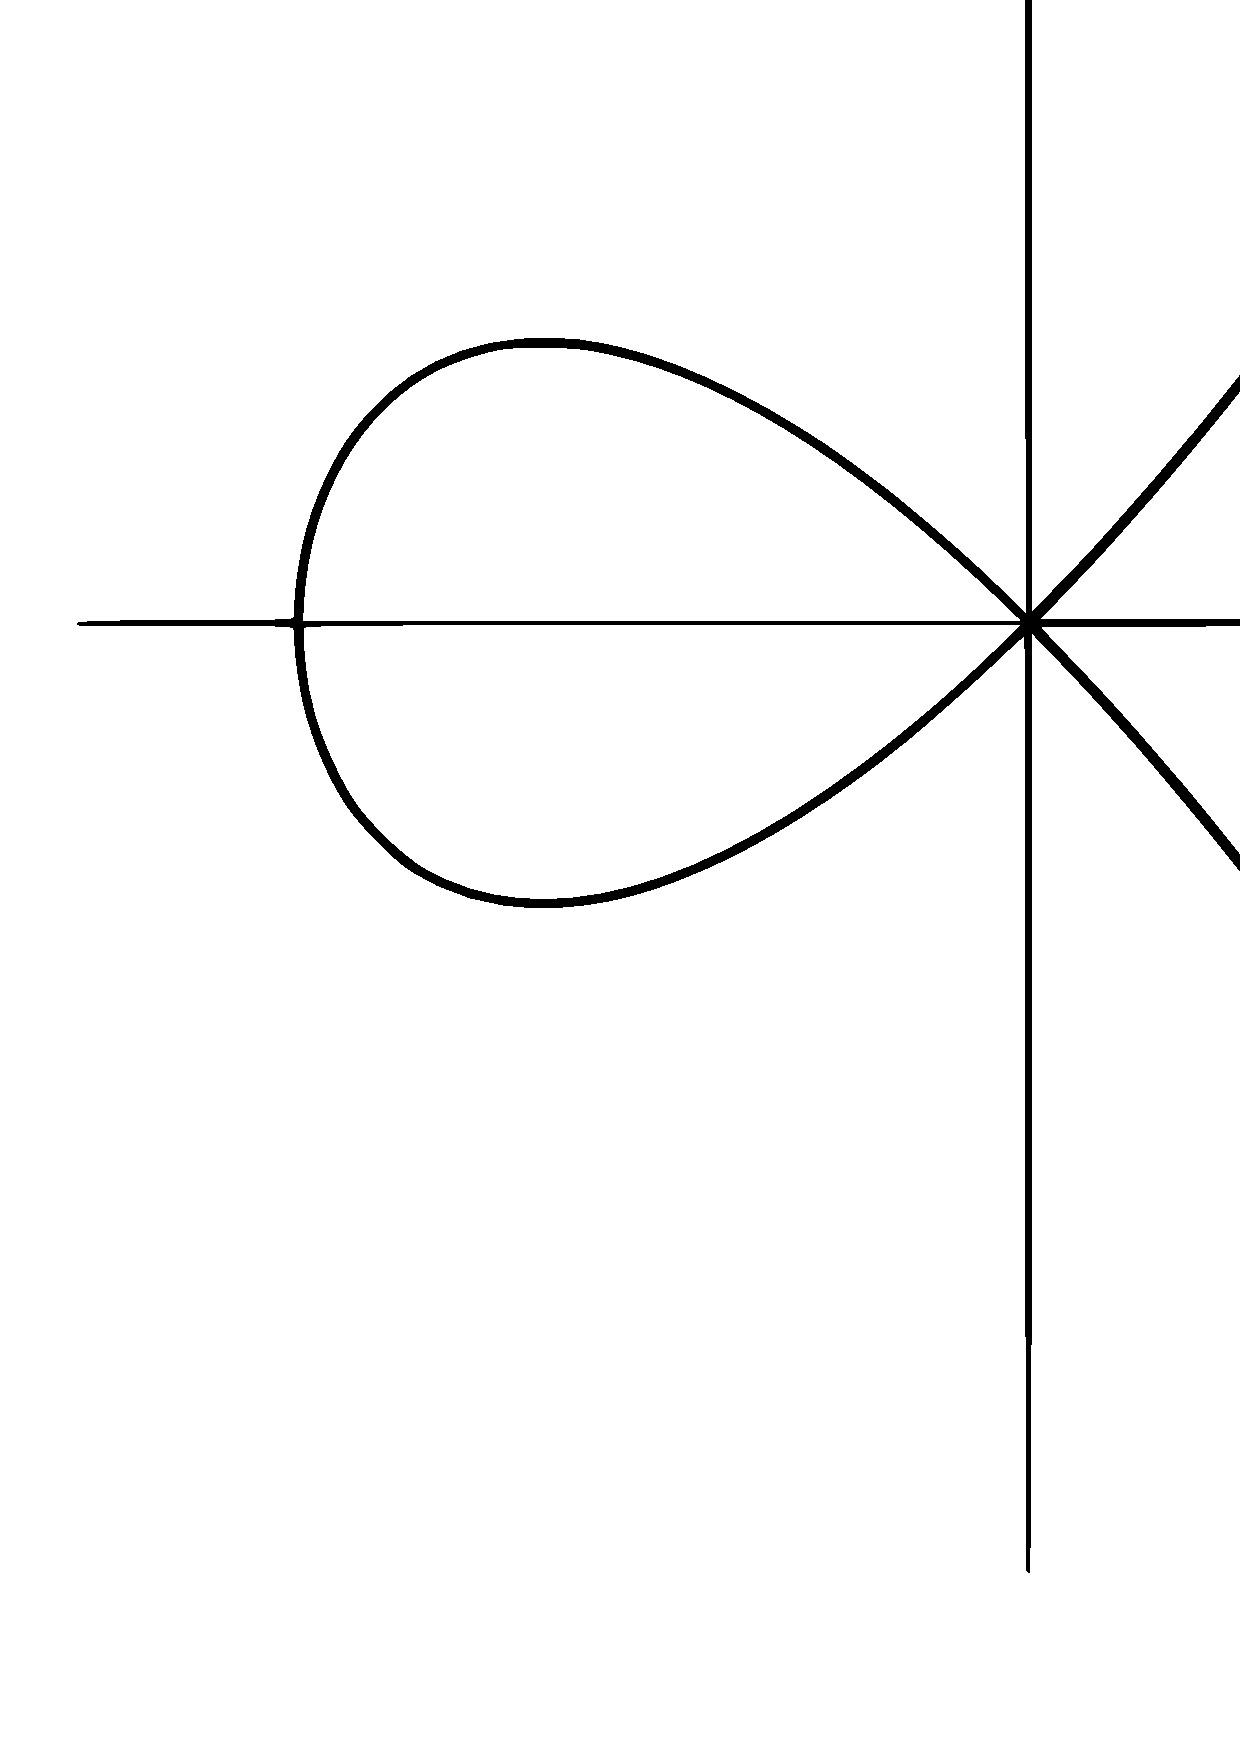
\includegraphics[scale=\scale,bb=0 0 668 462]{\PICDIR/2.png}\end{center}
\end{exe}

\begin{exe}\label{exe:3.9}
在上图中添入点$(4x_1-5x_0)$, $(2x_1-5x_0)$以及$(5)$的闭包(可以与第 \ref{s:2.4.3} 节中的$\mathbb A_{\mathbb Z}^2$的图相比较)。\textit{注意}:曲线$(4x_1-5x_0)$应该画得与“无穷远点”$(x_0)$相切,而曲线$(2x-5x_0)$不能。通俗地,我们可以说这是因为函数$5/4$在$(2)$处有一个双极点,而$5/2$只有一个单极点。(同样可见 Exercise \ref{exe:2.38} 中的讨论。)
\end{exe}

\begin{exe}\label{exe:3.10}
按上面的记号,令$h$为$S$的一个正次齐次元。集合
\[
	(\proj S)_h:=\proj S-V(h)
\]
同前为$S$中不包含$h$的齐次素理想构成的集合。证明这个集合依然一一对应于$S[h^{-1}]_0$的素理想,所以实际上存在一个$\spec S[h^{-1}]_0$与$\proj S$的(仿射)开子概形的同构。同样证明,这样的仿射开集族
\[
	\{(\proj S)_h\}_{h\in H}
\]
是一个$\proj S$的开覆盖,当且仅当$H$的元素生成了一个根为$S+$的理想。
\end{exe}

\begin{exe}\label{exe:3.11}
推广$\proj S$的定义到$S$不被$1$-次元所生成的情况,以及证明$\proj S$是一个射影概形。
\end{exe}

\begin{exe}\label{exe:3.12}
令$S$是一个分次环,没必要是有$1$-次元生成的。对任意的正次$d$,定义$S$的$d$-次\textit{Veronese 子环}为分次环
\[
	S^{(d)}=\bigoplus_{\nu=1}^\infty S_{d\nu}
\]
证明$\proj S$同构于$\proj S^{(d)}$. 然而,证明如果$S=A[x,y]$,则$S^{(d)}$作为分次代数(甚至仅作为环)并不同构于$S$. 于是,就像在簇中那样,分次代数与射影概形的对应并不是一一的。
\end{exe}

\subsection{\texorpdfstring{$\proj R$}{Proj R}的闭子概形}\label{s:3.2.2}

一个齐次理想$I\subset A[x_0$, $\dots$, $x_r]$确定了一个凝聚理想层$\tilde I\subset \mathscr O_{\mathbb P_A^r}$,因而一个$\mathbb P_A^r$的闭子概形。下面的习题建立了这些事实。

\begin{exe}\label{exe:3.13}
对每个开集
\[
	U_i=(\mathbb P_A^r)_{x_i}=\spec A[x_0,\dots,x_r,x_i^{-1}]_0\cong \mathbb A_A^r,
\]
令$\tilde I(U_i)$为理想$I\cdot A[x_0,\dots,x_r,x_i^{-1}]\cap A[x_0,\dots,x_r,x_i^{-1}]_0$. 证明这个定义可以以唯一的方式拓展到其他开集$U$上使得$\tilde{I}$成为一个凝聚理想层。所以我们称$\mathbb P_A^r$的闭子概形$V(\tilde{I})$\textit{关联于一个齐次理想$I$}.
\end{exe}

\begin{exe}\label{exe:3.14}
反之,给定一个$\mathbb P_A^r$的一个闭子概形,我们可以定义一个齐次理想$I(X)\subset A[x_0$, $\dots$, $x_r]$为齐次多项式$p(x_0,\dots,x_r)$生成的理想,其中齐次多项式需满足对每一个$i$,将其置于$1$后给出了元素
\[
	p(x_0,\dots,1,\dots,x_r)\in \mathscr I_X(U_i)\subset A[x_0,\dots,x_r,x_i^{-1}]_0.
\]
证明,如果$I=I(X)$,则$\tilde I=\mathscr I_X$.
\end{exe}

注意到连同 Exercise \ref{exe:3.7} ,它说明了每一个射影簇的闭子概形也是射影的:如果$I\subset S=A[x_0$, $\dots$, $x_r]$是一个齐次理想,则$V(\tilde{I})\subset \mathbb P^r_A$同构于概形$\proj S/I$.

\begin{exe}\label{exe:3.15}
子概形与理想的对应不再像仿射概形的情况是一一对应了。比如,证明在$\mathbb P_K^1$中,其中$K$是一个域,理想$I=(x_0)$和$I'=(x_0^2,x_0x_1)$都定义了同一个约态、单点子概形。更一般地,证明,如果$I\subset S=K[x_1$, $\dots$, $x_r]$是任意的齐次理想,以及对任意的整数$n_0$,通过
\[
	I'=\bigoplus_{n\geq n_0}I_n
\]
定义一个理想$I'\subset I$,则$I$和$I'$定义了$\mathbb P_K^r$的同一个子概形。
\end{exe}

\begin{exe}\label{exe:3.16}
为了解决这点,定义一个齐次理想$J\subset S:=A[x_0$, $\dots$, $x_r]$的\textit{饱和化}为理想
\[
	I=\{F\in S\,:\, \text{对某个$n$,$F\cdot S_n\subset J$}\},
\]
以及,称一个齐次理想是\textit{饱和}的,如果它等于它的饱和化。证明,存在一个$\mathbb P_A^r$的子概形与饱和理想之间的一一对应。
\end{exe}

\begin{exe}\label{exe:3.17}
证明,Exercise \ref{exe:3.12} 中的同构定义了一个射影空间$\mathbb P_A^r$以及$\mathbb P_A^N$的一个闭子概形之间的同构,其中$N=\dim_A(A[x_0$, $\dots$, $x_r]_d)$.(这就是概形版的Veronese映射。)
\end{exe}

\begin{exe}\label{exe:3.18}
证明,如果$R$是一个环$A=R_0$上的有限生成分次环(没必要是有其$1$-次元生成的),$\proj R$同构于某个射影空间$\mathbb P_A^r$的闭子概形。
\end{exe}

我们以一个定义和基本定理结束这一小节。

\begin{defi}
一个概形间态射$\varphi:X\to Y$被称为\textit{射影}的,如果他是一个闭嵌入$X\to \mathbb P_Y^n$和结构态射$\mathbb P_Y^n\to Y$的复合。
\end{defi}

注意到,如果$Y=\spec A$是仿射的,这相当于说$X$具有形式$\proj S$,其中$S$是一个有限生成$A$-代数。射影态射的基本事实前面已经说过了:

\begin{thm}\label{thm:3.20}
射影态射是逆紧的。
\end{thm}

证明可见Hartshorne [1977, Theorem II.4.9].

\begin{exe}\label{exe:3.21}
证明,有限态射$\varphi:X\to Y$是逆紧的且局部射影的,所谓局部射影即指,$Y$可以被开集族$U\subset Y$所覆盖,使得限制$\varphi:V=\varphi^{-1}U\to U$是射影的。(我们采用了 Hartshorn [1977, Section II.4] 中射影态射的定义,而在 Grothendieck [1961, EGA II, 5.5] 中,射影是指我们这里被叫做局部射影的性质。)
\end{exe}

\subsection{整体\texorpdfstring{$\proj$}{Proj}} \label{s:3.2.3}

\paragraph*{分次\texorpdfstring{$\oo_X$}{OX}-代数的层的\texorpdfstring{$\proj$}{Proj}}\addcontentsline{toc}{subsubsection}{分次\texorpdfstring{$\oo_X$}{OX}-代数的层的\texorpdfstring{$\proj$}{Proj}}
分次环$S$的$\proj$的构造给出了一个概形$X=\proj S$以及一个结构态射$X\to B=\spec(S_0)$. 因为$\proj S$与$S$的关联是函子性的,所以存在一个更一般的构造,给出概形$X$以及结构态射$X\to B$,其中$B$是任意概形,使得当$B$是仿射的时候将回到$\proj$:我们只需对一般的$B$,用$\oo_B$上的代数层代替分次$S_0$-代数$S$.

为实现这个构造,令$B$为任意概形,一个\textit{拟凝聚分次$\oo_B$-代数层}是指一个$B$上的拟凝聚代数层$\mathscr F$,具有一个分次
\[
	\mathscr F=\bigoplus_{\nu=0}^\infty \mathscr F_\nu
\]
使得$\mathscr F_\nu \mathscr F_\mu\subset \mathscr F_{\mu+\nu}$以及$\mathscr F_0=\oo_B$. 因此,对每一个仿射开集$U\subset B$,其坐标环为$A=\oo_B(U)$,环$\mathscr{F}(U)$是一个分次$A$-代数,其$0$次部分为$\mathscr F(U)_0=A$. 

给定这样一个层$\mathscr F$,对每个仿射开集$U\subset B$,我们令$X_U\to U$为概形$X_U=\proj \mathscr F(U)$及结构态射$\proj \mathscr F(U)\to \spec A=U$. 对每个$B$的开子集的含入$U\subset V$,限制映射$\mathscr F(V)\to \mathscr F(U)$是一个分次环的同态,其$0$次部分为限制映射$\oo_B(V)\to \oo_B(U)$,所以诱导了一个映射$X_U\to X_V$与结构态射$X_U\to U$和$X_V\to V$以及含入$U\hookrightarrow V$可交换。我们于是可以将概形$X_U$粘起来得到概形$X$,其具有结构态射$X\to B$,记作$\proj \mathscr F$,而$X$的构造则被称为\textit{整体$\proj$}.

就像在普通的$\proj$中一样,大部分情况下代数层$\mathscr F$由其$1$-次部分$\mathscr F_1$所生成,以及$\mathscr F_1$是凝聚的(或者,某种程度上更一般地,对某个$d>0$,Veronese 子层
\[
	\mathscr F^{(d)}=\bigoplus_{\nu=0}^\infty \mathscr F_{d\nu}
\]
由$\mathscr F_{d\nu}$所生成,而$\mathscr F_{d\nu}$是凝聚的
)。在这个假设下,同样如同普通的$\proj$,态射$\proj \mathscr F\to B$是逆紧的。

整体$\proj$最简单的例子给了我们任意概形$S$上的射影空间的另一个构造。回忆在第 \ref{chap:1} 章,任意概形$S$上的射影空间是黏合构造而成的:如果$S$被仿射概形族$U_\alpha=\spec R_\alpha$所覆盖,我们定义射影空间$\mathbb P_S^n$为射影空间$\mathbb P_{U_\alpha}^n$的并,并通过$U_\alpha\cap U_\beta$上的恒等映射诱导的黏合映射粘起来。我们也可以通过乘积来定义它:
\[
	\mathbb P_S^n=\mathbb P_{\mathbb Z}^n\times_{\spec \mathbb Z}S.
\]
最后,我们可以将其实现为$S$上秩为$n+1$的自由层的对称代数的整体$\proj$:

\begin{exe}\label{exe:3.22}
令$S$为任意概形。证明$S$上的射影空间$\mathbb P_S^n$可以由整体$\proj$构造:
\[
	\mathbb P_S^n=\proj \left(\operatorname{Sym}(\oo_S^{\oplus n+1})\right).
\]
\end{exe}

特别地,在纤维积外,我们可以将给定概形$S$上的射影空间的乘积同构整体$\proj$实现:如果我们记$\oo_{\mathbb P_S^r}[X_0$, $\dots$, $X_m]$为分次$\oo_{\mathbb P_S^n}$-代数层$\operatorname{Sym}\left(\oo_{\mathbb P_S^n}^{\oplus m+1}\right)$,则
\[
	\mathbb P^n_S\times_S \mathbb P^m_S=\proj \oo_{\mathbb P^n_S}[X_0,\dots,X_m].
\]
第三种方式是通过\textit{Segre嵌入}:

\begin{exe}\label{exe:3.23}
令$S$为任意概形。证明
\begin{align*}
\mathbb P_S\times_S \mathbb P_S^m &\cong V\left(\{X_{i,j}X_{k,l}-X_{i,l}X_{k,j}\}\right)\subset \proj \oo_S[\{X_{i,j}\}_{0\leq i\leq n;0\leq j\leq m}]\\
& = \mathbb P_S^{(n+1)(m+1)-1}.
\end{align*}
\end{exe}

于是,至少局部地在基上,这给了我们一种方式来描述这样乘积的子概形:

\begin{exe}\label{exe:3.24}
令$S=\spec R$为任意的仿射概形。证明
\[
	X\subset \proj R[x_0,\dots,x_n]\times_S \proj R[y_0,\dots,y_m]=\mathbb P^n_S\times_S\mathbb P^m_S
\]
任意的闭子概形都可以由族$\{F_\alpha(x_0$, $\dots$, $x_n;y_0$, $\dots$, $y_m)\}$的零点集给出,其中$F_{\alpha}$是两族变量$(x_0$, $\dots$, $x_n)$和$(y_0$, $\dots$, $y_m)$的齐次函数。特别地,证明矩阵
$
\begin{pmatrix}
x_0&x_1&\cdots &x_n\\
y_0&y_1&\cdots &y_n\\
\end{pmatrix}
$
的$2\times 2$子式的理想定义了$\mathbb P^n_S\times_S\mathbb P^m_S$中的对角集。推出任意射影态射都是可分的。
\end{exe}

整体$\proj$构造的一个更严肃的应用是定义概形$X$沿着闭子概形$Y\subset X$的\textit{爆破},我们将在第 \ref{chap:5} 章中完整地讨论它。整体$\proj$另一个通常的应用是我们下面描述的矢量丛的射影化。

\paragraph*{凝聚层\texorpdfstring{$\mathscr E$}{E}的射影化\texorpdfstring{$\mathbb P(\mathscr E)$}{P(E)}}\addcontentsline{toc}{subsubsection}{凝聚层\texorpdfstring{$\mathscr E$}{E}的射影化\texorpdfstring{$\mathbb P(\mathscr E)$}{P(E)}}
我们在 Exercise \ref{exe:3.22} 中看到,

\nottran


\subsection{切空间和切锥} \label{s:3.2.4}
\paragraph*{仿射与射影切空间}\addcontentsline{toc}{subsubsection}{仿射与射影切空间}
一个概形的Zariski切空间是抽象矢量空间。但当一个$K$上的概形$X$被嵌入到一个环绕空间中,比如$K$上的仿射或射影空间,我们可以将$X$的一个剩余类域为$K$的点$p$关联于对应仿射或者射影空间的线性子簇,其被称为$X$在点$p$的\textit{仿射切空间}或\textit{射影切空间}。

\subsection{到射影空间的态射} \label{s:3.2.5}
\subsection{分次模和层} \label{s:3.2.6}
\subsection{Grassmann流形} \label{s:3.2.7}
\subsection{全景超曲面} \label{s:3.2.8}
